\chapter{极限与连续}
\label{chap:limits-continuity}
\label{chap:function-limits}
\label{chap:mathematical-analysis}

第~\ref{chap:sets-relations-maps}章的等比递推给出了有限步结果$e^{(t)}=\rho^te_0$，上一章又算出了有限几何和与裂项和。
当$t$或项数无限增大时，这些数是否趋向确定的值？输入无限靠近某一点时，函数值又趋向哪里？
回答这类问题，先要说清“趋近”的含义，再判断在什么条件下趋近确实产生一个确定的结果，以及这种结果能否与加减乘除、复合等运算交换次序。

本章的主线从数列出发。数列极限用误差条件定义，我们分别讨论已知收敛时怎样计算极限、不知道极限值时怎样保证极限存在，后者要用到上一章的确界原理。
级数是部分和组成的数列，数列的结论由此用于无限多项的累计，并引出重排与分组这些有限和中不会出现的问题。
随后把极限推广到实变量函数，用函数极限定义连续性，并在闭区间上证明最值、介值和一致连续这几条整体性质。
最后一步让函数本身随编号变化：函数列与函数项级数何时保持连续性，以及幂级数在哪些输入处收敛。
本章只使用实轴上的距离$|x-y|$，一般距离下的相应理论在第~\ref{chap:metric-spaces}章统一讨论。

\section{数列的极限}
\label{sec:ru-sequence-limits}
\label{sec:analysis-continuous-limits}
\label{sec:analysis-sequences-series-errors}

数列$1,1/2,1/3,\ldots$越来越接近$0$，数列$-1,1,-1,1,\ldots$则在两个值之间来回交替。
直觉上前者“有极限”，后者没有；但“越来越接近”需要精确的含义，否则无法判断$(1+1/n)^n$或$\sum_{k\leq n}1/k$这类数列是否趋向某个数。
本节先用误差条件定义收敛并建立极限的运算，再给出不必事先知道极限值的存在性判别，最后描述趋向无穷和不收敛数列的尾部行为。

\subsection{收敛、发散与极限运算}
\label{sec:ru-convergence-limit-laws}

比较$(1/n)$与$((-1)^n)$，区别在于尾部。$1/n$从某一项起全部落在$0$附近任意窄的范围内；$((-1)^n)$的偶数项都等于$1$，奇数项却始终离$1$有距离$2$。
所以“接近一个数”必须约束后面的\emph{每一项}。只要求“各项离$a$越来越近”也不够：$1+1/n$离$0$越来越近，却始终大于$1$。
合适的要求是：无论事先给定多小的正误差，从某一项起，后面每一项与$a$的距离都小于这个误差。

\begin{definition}[数列的极限]
\label{def:ru-sequence-limit}
设$(a_n)$为实数列，$a\in\mathbb R$。若对每个$\varepsilon>0$，都存在正整数$N$，使
\[
 n\geq N\quad\Longrightarrow\quad|a_n-a|<\varepsilon,
\]
就称$(a_n)$\term{收敛}（converge）到$a$，$a$称为它的极限，记作$\lim_{n\to\infty}a_n=a$或$a_n\to a$。没有实数极限的数列称为\term{发散}（diverge）。
\end{definition}

定义中的量词次序不能交换：先任给误差$\varepsilon$，再选取尾部起点$N$。$N$可以依赖于$\varepsilon$，误差要求越严格，所需的起点通常越靠后。
极限也不要求某一项恰好等于$a$\scite{math-lebl-analysis1}。
例如对$a_n=1/n$，任给$\varepsilon>0$，由Archimedes性取正整数$N>1/\varepsilon$，则$n\geq N$时$|1/n-0|\leq1/N<\varepsilon$，所以$1/n\to0$。
图~\ref{fig:analysis-process-sequence-tail}把“全部尾部项”画成同一条误差带。

\begin{figure}[!htbp]
 \centering
 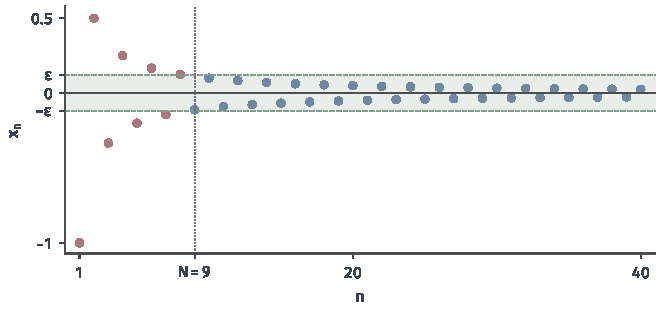
\includegraphics[width=112.0mm]{figures/01-mathematical-preliminaries-upper/00-shared/matplotlib/chapter3-concept-processes/sequence-tail.pdf}
 \caption{数列$x_n=(-1)^n/n$的前40项。绿色带为$|x_n|<0.12$，取$N=9$后，所有$n\geq9$都在带内；蓝点标记这个尾部，红点标记之前的项。尾部条件针对无限多个$n$，其成立依据是$1/n\leq1/9<0.12$，不是只检查图中有限个点。}
 \label{fig:analysis-process-sequence-tail}
\end{figure}

要说明$a_n$不收敛到$a$，须写出定义的否定：存在某个$\varepsilon_0>0$，使得无论$N$取多大，总有$n\geq N$满足$|a_n-a|\geq\varepsilon_0$。
对$((-1)^n)$，取$\varepsilon_0=1$：相邻两项相差$2$，不可能同时落在长度为$2$的开区间$(a-1,a+1)$内，所以它不收敛到任何$a$，是发散数列。

定义需要先给出一个候选极限$a$，那么会不会有两个候选都满足定义？不会。若$a\neq b$都是极限，取$\varepsilon=|a-b|/3$，充分靠后的项同时满足$|a_n-a|<\varepsilon$和$|a_n-b|<\varepsilon$，
三角不等式却给出$|a-b|\leq|a-a_n|+|a_n-b|<2|a-b|/3$，矛盾。所以收敛数列的极限唯一，记号$\lim a_n$表示一个确定的数。

定义只控制尾部，而尾部之前只有有限个项，因此收敛数列必有界。设$a_n\to a$，取$\varepsilon=1$得到$N$，使$n\geq N$时$|a_n|<|a|+1$；
再令$M=\max\{|a_1|,\ldots,|a_{N-1}|,|a|+1\}$，就有$|a_n|\leq M$对所有$n$成立。
反过来不成立，$((-1)^n)$有界却不收敛。这一性质常以逆否形式使用：无界数列一定发散。

已知几个数列收敛时，由它们组合出的数列的极限可以直接算出。思路都是把新数列的误差拆成已知误差的组合。
\begin{theorem}[数列极限的四则运算]
\label{thm:ru-sequence-limit-laws}
设$a_n\to a$，$b_n\to b$，其中$a,b\in\mathbb R$，$c$为实常数，则
\[
 a_n\pm b_n\to a\pm b,\qquad ca_n\to ca,\qquad a_nb_n\to ab.
\]
若还有$b\neq0$，则充分靠后的$b_n\neq0$，并且$a_n/b_n\to a/b$。
\end{theorem}
\begin{proof}
和与差由$|(a_n\pm b_n)-(a\pm b)|\leq|a_n-a|+|b_n-b|$得到：让两个误差各小于$\varepsilon/2$即可。数乘的误差是$|c|\,|a_n-a|$，同样可以任意小。

乘积的误差含有一个变化的因子，需要用到收敛数列的有界性。取$M\geq1$使所有$|a_n|\leq M$，则
\[
 |a_nb_n-ab|=|a_n(b_n-b)+b(a_n-a)|\leq M|b_n-b|+|b|\,|a_n-a|,
\]
让$|b_n-b|<\varepsilon/(2M)$与$|a_n-a|<\varepsilon/[2(|b|+1)]$同时成立，右侧便小于$\varepsilon$。

对商，先取误差$|b|/2$，得知充分靠后的$|b_n|\geq|b|/2>0$。于是
\[
 \Bigl|\frac1{b_n}-\frac1b\Bigr|=\frac{|b_n-b|}{|b_n|\,|b|}\leq\frac{2|b_n-b|}{|b|^2}\to0,
\]
前面有限个项不影响极限，再对$a_n\cdot(1/b_n)$用乘积规则。
\end{proof}
例如把分子分母同除以$n$，得$n/(n+1)=1/(1+1/n)\to1$。分母极限为零时不能套用商的规则：$0/0$与$\infty-\infty$都不是可以直接计算的数值，须先变形。

有时一个数列不断振荡，直接控制它的误差并不方便，但能找到两个趋向同一值的上下界。
\begin{theorem}[夹逼定理]
\label{thm:analysis-sequence-squeeze}
设实数列满足：存在$N_0$使$n\geq N_0$时$a_n\leq c_n\leq b_n$，并且$a_n\to\ell$、$b_n\to\ell$，其中$\ell\in\mathbb R$，则$c_n\to\ell$。
\end{theorem}
\begin{proof}
任给$\varepsilon>0$，取$N\geq N_0$使$n\geq N$时$|a_n-\ell|<\varepsilon$且$|b_n-\ell|<\varepsilon$。于是$\ell-\varepsilon<a_n\leq c_n\leq b_n<\ell+\varepsilon$，即$|c_n-\ell|<\varepsilon$。
\end{proof}
例如$-1/n\leq(\sin n)/n\leq1/n$，所以$(\sin n)/n\to0$。

等比数列$(r^n)$是反复出现的例子，夹逼定理可以判定它的全部情形。$r=0$时显然趋于零。若$0<|r|<1$，写$1/|r|=1+h$，$h>0$。
对$n$归纳可证$(1+h)^n\geq1+nh$：$n=1$时取等号；若对$n$成立，则$(1+h)^{n+1}\geq(1+nh)(1+h)\geq1+(n+1)h$。
因此$0<|r|^n\leq1/(1+nh)<1/(nh)\to0$，再对$-|r|^n\leq r^n\leq|r|^n$用夹逼定理，得到$r^n\to0$。
$r=1$时各项恒为$1$，收敛；$r=-1$时在$\pm1$间交替，发散；$|r|>1$时同一不等式给出$|r|^n\geq1+nh$（其中$|r|=1+h$），数列无界，因而发散。
回到等比递推~\eqref{eq:prelim-geometric-recurrence}：设$e_0\neq0$，$e^{(t)}=\rho^te_0$恰在$|\rho|<1$时趋于零，在$\rho=1$时保持不变，其余情形发散。

\subsection{极限存在的判别}
\label{sec:ru-limit-existence}

定义收敛时需要先给出候选极限，但很多数列的极限值事先并不知道。下面依次利用变化方向、取值范围和尾部各项的相互接近来判断极限是否存在。

若对所有$n$都有$a_n\leq a_{n+1}$，称数列单调不减；若总有$a_n\geq a_{n+1}$，称数列单调不增，两者统称单调数列。
单调不减且有上界的数列，全部项的集合有上确界；单调性又保证后面的项一直靠近它。
\begin{theorem}[单调有界收敛定理]
\label{thm:analysis-monotone-bounded-sequence}
单调不减且有上界的实数列收敛，极限为$\sup\{a_n:n\geq1\}$；单调不增且有下界的实数列收敛，极限为$\inf\{a_n:n\geq1\}$。
\end{theorem}
\begin{proof}
设$a=\sup\{a_n:n\geq1\}$，它由确界原理保证存在。给定$\varepsilon>0$，$a-\varepsilon$不是上界，所以存在$N$使$a_N>a-\varepsilon$。
单调性使$n\geq N$时$a-\varepsilon<a_N\leq a_n\leq a$，这正是$a_n\to a$。单调不增的情形对$-a_n$应用同一论证。
\end{proof}
两个条件都不能省去：$(n)$单调却无上界，$((-1)^n)$有界却不单调。结合收敛数列的有界性，单调数列收敛当且仅当它有界。

有界数列未必收敛，但其中可能有一部分项具有共同的趋向。若$n_1<n_2<\cdots$为严格递增的正整数列，则$(a_{n_k})_{k\geq1}$称为$(a_n)$的\term{子列}（subsequence），由归纳可知$n_k\geq k$。
收敛数列的每个子列都收敛到同一极限：若$n\geq N$时$|a_n-a|<\varepsilon$，则$k\geq N$时$n_k\geq k\geq N$，同一误差界仍然适用。
\begin{theorem}[Bolzano--Weierstrass定理]
\label{thm:analysis-bounded-subsequence}
有界实数列必有收敛子列。
\end{theorem}
\begin{proof}
设$|a_n|\leq M$。从包含全部项的闭区间$I_0=[-M,M]$出发，将它平分；两半中至少有一半含有无穷多个下标对应的项，选出这一半。
重复平分与选择，得到嵌套闭区间$I_0\supseteq I_1\supseteq\cdots$，其中每个$I_k$都含有无穷多项，长度为$2M\cdot2^{-k}$。
由于每个$I_k$都含有无穷多项，可以依次选取下标$n_1<n_2<\cdots$使$a_{n_k}\in I_k$。
由$2^k\geq k+1$，区间长度可以任意小，闭区间套性质给出唯一公共点$c$。$a_{n_k}$与$c$都在$I_k$中，所以$|a_{n_k}-c|\leq2M\cdot2^{-k}\to0$。
\end{proof}
“有界”只能保证子列收敛，不能保证整列收敛：$((-1)^n)$的偶数项子列收敛到$1$，奇数项子列收敛到$-1$，整列却发散。

单调条件并不适用于所有收敛数列。不知道候选极限时，还可以检查尾部各项是否彼此接近。满足
\[
 \forall\varepsilon>0,\quad\exists N,\quad\forall m,n\geq N,\quad|a_m-a_n|<\varepsilon
\]
的数列称为\term{柯西数列}（Cauchy sequence）。这个条件只涉及数列自身的项，不需要知道极限是多少。
\begin{theorem}[柯西收敛准则]
\label{thm:analysis-cauchy-convergence}
实数列收敛，当且仅当它是柯西数列。
\end{theorem}
\begin{proof}
收敛数列是柯西数列：若$n\geq N$时$|a_n-a|<\varepsilon/2$，则对$m,n\geq N$有$|a_m-a_n|\leq|a_m-a|+|a-a_n|<\varepsilon$。

反过来，先说明柯西数列有界：取误差$1$得到$N$，所有$n\geq N$都满足$|a_n-a_N|<1$，前面有限项另取最大绝对值即可。
由Bolzano--Weierstrass定理，可取子列$a_{n_k}\to a$。给定$\varepsilon>0$，选$N$使$m,n\geq N$时$|a_m-a_n|<\varepsilon/2$，再选$k$使$n_k\geq N$且$|a_{n_k}-a|<\varepsilon/2$。
于是每个$n\geq N$都有$|a_n-a|\leq|a_n-a_{n_k}|+|a_{n_k}-a|<\varepsilon$。
\end{proof}
充分性经过收敛子列，因而仍然依赖确界原理。在有理数中，$\sqrt2$的十进制截断$1,1.4,1.41,\ldots$是柯西数列，却没有有理数极限。

验证柯西条件时，可把两个较晚的项之间的距离估计为逐步变化的总和：对$m>n$，
\begin{equation}
 |a_m-a_n|\leq\sum_{k=n}^{m-1}|a_{k+1}-a_k|.
 \label{eq:analysis-cauchy-tail-bound}
\end{equation}
只看相邻两项不够，因为中间的步数也在增加。设$a_1=0$、$a_{k+1}-a_k=1/k$，每一步都趋于零；但$a_{2n}-a_n=\sum_{k=n}^{2n-1}1/k$共有$n$项，每项都大于$1/(2n)$，
所以$a_{2n}-a_n>1/2$。它不是柯西数列，因而发散。这里的$a_{n+1}$正是第~\ref{sec:analysis-series}节调和级数的前$n$项和。

\subsection{无穷极限、上极限与下极限}
\label{sec:ru-infinite-limits-limsup}

数列$(n)$发散，但它的发散方式很确定：越过任何有限界以后不再回头。为记录这种趋向，规定$a_n\to+\infty$表示对每个实数$M$，都存在$N$使$n\geq N$时$a_n>M$；
$a_n\to-\infty$则要求最终都有$a_n<M$。趋向$\pm\infty$的数列仍是发散数列，$\pm\infty$不是实数极限。
把这两个符号加入实数，得到扩展实数$\overline{\mathbb R}=\mathbb R\cup\{-\infty,+\infty\}$。其中的运算只在不引起歧义时定义，例如$a+(+\infty)=+\infty$（$a$为实数）；
$\infty-\infty$、$0\cdot\infty$与$\infty/\infty$都没有定义，因为不同的数列组合会给出不同结果，如$(n+1)-n\to1$而$2n-n\to+\infty$。

不收敛的数列仍然可以考察尾部的上下边界。逐渐舍去前项时，尾部下确界只会上升，尾部上确界只会下降，因此可以用单调数列的极限记录它们。
\begin{definition}[上极限与下极限]
\label{def:analysis-liminf-limsup}
对实数列$(a_n)$，定义
\[
 \liminf_{n\to\infty}a_n=\lim_{n\to\infty}\inf_{k\geq n}a_k,\qquad
 \limsup_{n\to\infty}a_n=\lim_{n\to\infty}\sup_{k\geq n}a_k,
\]
分别称为\term{下极限}（limit inferior）与\term{上极限}（limit superior）。尾部无上界时$\sup_{k\geq n}a_k=+\infty$，无下界时尾部下确界为$-\infty$。
\end{definition}
右侧尾部下确界随$n$单调不减，尾部上确界随$n$单调不增，所以两个极限都在扩展实数中存在：单调有界时由单调有界收敛定理得到有限极限，无界时趋于相应的无穷。
每个尾部的下确界不超过同一尾部的上确界，所以总有$\liminf a_n\leq\limsup a_n$。

上、下极限恰好刻画了通常的收敛。若二者都等于有限数$a$，给定$\varepsilon>0$，充分靠后的尾部下确界大于$a-\varepsilon$、尾部上确界小于$a+\varepsilon$，
夹在中间的每个尾部项都满足$|a_n-a|<\varepsilon$，即$a_n\to a$。反之若$a_n\to a$，则$n\geq N$时尾部全落在$(a-\varepsilon,a+\varepsilon)$内，尾部的上下确界都在$[a-\varepsilon,a+\varepsilon]$中。
同理，两者都等于$+\infty$恰好对应$a_n\to+\infty$，都等于$-\infty$对应$a_n\to-\infty$。

两者不相等时，它们记录了数列尾部来回摆动的范围。$((-1)^n)$的下极限为$-1$、上极限为$1$；$((-1)^nn)$的下极限为$-\infty$、上极限为$+\infty$；
$(n(1+(-1)^n))$的奇数项为$0$、偶数项为$2n$，下极限为$0$、上极限为$+\infty$。
对有界数列，上极限还是某个子列的极限：记$L=\limsup a_n$，对每个$j$先取足够晚的起点使其后的尾部上确界小于$L+1/j$，
这一尾部中又有某项大于$L-1/j$；在超过前次所选下标的位置选出这样的项，便得到趋于$L$的子列。下极限同理。

\section{级数的极限}
\label{sec:ru-series}
\label{sec:analysis-series}

有限和可以逐项相加，无限多项却无法“加完”。上一节的数列极限提供了处理办法：把前$N$项的和看成一个数列，再问$N$无限增大时它是否趋向确定的数。
本节先用部分和定义级数及其和，计算几类可作基准的级数；随后建立收敛判别，区分不依赖抵消的绝对收敛与依赖抵消的条件收敛；最后说明改变求和次序或合并相邻项会怎样影响结果。

\subsection{部分和、余项与基本级数}
\label{sec:ru-partial-sums}
\label{sec:analysis-series-definition}

给定数列$(a_n)_{n\geq1}$，称$s_N=\sum_{n=1}^Na_n$为第$N$个\term{部分和}（partial sum）。符号\term{无穷级数}（infinite series）$\sum_{n=1}^\infty a_n$描述这一求和过程；
若部分和数列$(s_N)$有有限极限$s$，称级数收敛，并记$\sum_{n=1}^\infty a_n=s$，称$s$为级数的和；否则称级数发散。
三个对象要分清：单项$a_n$、部分和$s_N$与级数的和$s$。例如$a_n=2^{-n}\to0$，而$s_N=1-2^{-N}\to1$。

由$a_N=s_N-s_{N-1}$及差的极限法则，级数收敛必须有$a_N\to0$。反向不成立：上一节末尾的例子说明调和级数$\sum1/n$的单项趋于零，部分和却不是柯西数列，因而发散。

级数是否收敛与前有限项无关，因为删去前$m$项只让部分和相差固定的$s_m$。级数收敛时，$r_N=s-s_N=\sum_{n>N}a_n$称为\term{余项}（remainder），它衡量截断到第$N$项的误差，并且$r_N\to0$。

\paragraph{基准级数}
几何级数与裂项级数的部分和可以直接写出，因而能算出级数的和与余项。由上一章的有限几何和，$|r|<1$时$r^{N+1}\to0$，于是
\begin{equation}
 \sum_{n=0}^\infty r^n=\frac1{1-r},\qquad \Bigl|\sum_{n=N+1}^\infty r^n\Bigr|=\frac{|r|^{N+1}}{|1-r|}.
 \label{eq:analysis-geometric-series}
\end{equation}
$|r|\geq1$时$|r^n|\geq1$，单项不趋零，级数发散。若$a_n=b_n-b_{n+1}$，裂项公式给出$s_N=b_1-b_{N+1}$，所以级数收敛当且仅当$(b_n)$有有限极限。

例如$\sum_{n=1}^\infty\frac1{n(n+1)}=1$，截断到第$N$项的余项恰为$1/(N+1)$。几何级数的余项按公比的幂衰减，裂项级数的余项按$1/N$衰减，后面比较其他级数时，这两种速度都会用到。

若所有$a_n\geq0$，部分和单调不减，由单调有界收敛定理，级数收敛当且仅当部分和有上界；无上界时部分和趋于$+\infty$。
因此对非负项级数统一记
\[
 \sum_{n=1}^\infty a_n=\sup_N\sum_{n=1}^Na_n\in[0,+\infty],
\]
称为非负项级数的扩展总和。总和为$+\infty$时仍称级数发散，但这个记号总有意义，后面比较、重排非负项时可以先在$[0,+\infty]$中比较总和。

\paragraph{$p$级数}
单调性给出了判断$p$级数$\sum_{n=1}^\infty n^{-p}$的办法。设$p>0$，按$n=2^k,\ldots,2^{k+1}-1$分块，每块有$2^k$项，块内每项介于$(2^{k+1})^{-p}$与$(2^k)^{-p}$之间，于是
\[
 2^{-p}\,2^{k(1-p)}\leq\sum_{n=2^k}^{2^{k+1}-1}n^{-p}\leq2^{k(1-p)}.
\]
任一部分和$s_N$都不超过前若干整块之和，所以只需估计整块。

$p>1$时右侧是公比$2^{1-p}<1$的几何级数，每个部分和都不超过$1/(1-2^{1-p})$，级数收敛；
$0<p\leq1$时每块至少为$2^{-p}$，累计任意多块便无界，级数发散；$p\leq0$时单项不趋零。
所以$p$级数恰在$p>1$时收敛，特别地，调和级数发散。这一论证只比较有限个区块，不需要积分判别法。

\subsection{级数极限存在的判别}
\label{sec:ru-series-tests}
\label{sec:analysis-series-tests}

判断级数收敛，就是判断部分和是否有有限极限。非负项的部分和单调，可以用已知级数的上界控制；出现正负项后，还须区分绝对值累计有限与依靠抵消才收敛这两种情形。

\begin{theorem}[正项级数的比较判别]
\label{thm:ru-series-comparison}
设充分大的$n$都有$0\leq a_n\leq b_n$。若$\sum b_n$收敛，则$\sum a_n$收敛；若$\sum a_n$发散，则$\sum b_n$发散。
若$a_n,b_n>0$且$a_n/b_n\to c\in(0,+\infty)$，则两级数同时收敛或同时发散。
\end{theorem}
\begin{proof}
第一句来自非负部分和的单调性：$\sum a_n$的部分和被$\sum b_n$的部分和控制，有限个前项不影响结论。
第二句称为极限比较判别：最终有$(c/2)b_n\leq a_n\leq(3c/2)b_n$，再用第一句。
\end{proof}
例如$\frac{1}{n^2+n}\leq\frac1{n^2}$，而$\frac{2n+1}{n^3}$与$\frac1{n^2}$之比趋于$2$，两者都收敛。

比较判别要求先找到合适的基准。用几何级数作基准，可以得到只看单项本身的判别法。设$a_n>0$。
\begin{theorem}[比值判别与根值判别]
\label{thm:ru-ratio-root-tests}
若$a_{n+1}/a_n\to q$，则$q<1$时$\sum a_n$收敛，$q>1$时发散。若$\limsup a_n^{1/n}=q$，结论相同。
\end{theorem}
\begin{proof}
比值情形：$q<1$时取$q<\rho<1$，充分靠后有$a_{n+1}\leq\rho a_n$，逐次代入得$a_{N+j}\leq a_N\rho^j$，与几何级数比较即收敛；$q>1$时充分靠后的项递增，不趋于零，级数发散。
根值情形：$q<1$时取$q<\rho<1$，由上极限的定义，充分靠后的尾部上确界小于$\rho$，于是$a_n<\rho^n$，与几何级数比较；$q>1$时有无穷多个$n$使$a_n^{1/n}>1$，即$a_n>1$，单项不趋零。
\end{proof}
两种判别在$q=1$时都没有结论：$\sum1/n$发散而$\sum1/n^2$收敛，它们的比值和$n$次根都趋于$1$。这时只能回到比较等更精细的方法。
以上判别都要求各项非负；对一般级数，可以先把它们用于$\sum|a_n|$。

\paragraph{绝对收敛与条件收敛}
若$\sum|a_n|$收敛，称$\sum a_n$\term{绝对收敛}（absolute convergence）。它的意思是：即使不依赖正负抵消，各项的绝对贡献之和也有限。
\begin{theorem}[绝对收敛蕴含收敛]
\label{thm:ru-absolute-convergence}
若$\sum|a_n|$收敛，则$\sum a_n$收敛，其和$s$满足$|s-s_N|\leq\sum_{n>N}|a_n|$。
\end{theorem}
\begin{proof}
对$m>n$，
\[
 |s_m-s_n|\leq\sum_{k=n+1}^m|a_k|\leq\sum_{k>n}|a_k|,
\]
右侧是收敛非负级数的余项，与$m$无关且随$n$增大趋于零，所以$(s_n)$满足柯西准则。令$m\to\infty$即得误差界。
\end{proof}
例如$\sum(-1)^{n+1}/n^2$由$p=2$的情形绝对收敛，截断到第$N$项的误差不超过$\sum_{n>N}1/n^2\leq\sum_{n>N}\frac1{n(n-1)}=\frac1N$。

若原级数收敛，而$\sum|a_n|$发散，称为\term{条件收敛}（conditional convergence）。这需要同时证明两件事；只知道绝对值级数发散，不能排除原级数也发散。
最基本的依靠抵消而收敛的情形是交错级数。
\begin{theorem}[交错级数的Leibniz判别]
\label{thm:ru-leibniz}
若$b_n\geq0$单调不增且$b_n\to0$，则$\sum_{n=1}^\infty(-1)^{n+1}b_n$收敛，其和$s$满足$|s-s_N|\leq b_{N+1}$。
\end{theorem}
\begin{proof}
偶数部分和$s_{2n+2}=s_{2n}+(b_{2n+1}-b_{2n+2})$单调不减，奇数部分和$s_{2n+1}=s_{2n-1}-(b_{2n}-b_{2n+1})$单调不增，并且每个偶数部分和都不超过任何奇数部分和。
所以两列分别有界单调，各自收敛；它们之差$s_{2n+1}-s_{2n}=b_{2n+1}\to0$，两个极限相同，记为$s$。给定误差后，奇偶两类下标的尾部分别满足要求，取较晚的起点即知$s_N\to s$。
$s$位于任意一对相邻部分和$s_N,s_{N+1}$之间，因此$|s-s_N|\leq|s_{N+1}-s_N|=b_{N+1}$。
\end{proof}
例如交错调和级数$\sum(-1)^{n+1}/n$收敛，绝对值级数却是调和级数，所以它条件收敛。若$\sum b_n$本身收敛，Leibniz条件给出的交错级数则是绝对收敛的，不能一概称为条件收敛。
图~\ref{fig:analysis-process-series-terms-sums}并排比较调和级数与交错调和级数：两者的项都趋于零，累计后的行为却不同。

\begin{figure*}[!htbp]
 \centering
 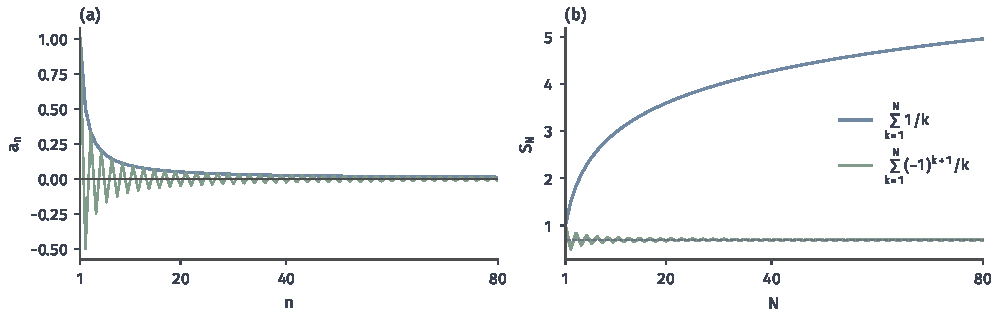
\includegraphics[width=169.0mm]{figures/01-mathematical-preliminaries-upper/00-shared/matplotlib/chapter3-concept-processes/series-terms-sums.pdf}
 \caption{(a) 蓝、绿折线分别连接$1/n$与$(-1)^{n+1}/n$的前80项。(b) 对应的部分和：调和部分和继续增长，交错调和部分和趋于虚线所示的$\log2$。项趋零只是级数收敛的必要条件；图展示有限段，收敛或发散由正文中的判别证明。}
 \label{fig:analysis-process-series-terms-sums}
\end{figure*}

\paragraph{Dirichlet判别}
交错级数的论证可以推广：若一列数的部分和有界振荡，再配上单调趋零的权重，乘积级数仍收敛。这一推广称为Dirichlet判别，作为补充推导列在这里，第~\ref{sec:ru-power-series-uniform}节证明幂级数在端点附近的一致收敛时要用到同样的技巧。

设$A_N=\sum_{n=1}^Na_n$满足$|A_N|\leq M$，$b_n\geq0$单调趋零。对$m\leq k$记$A^{(m)}_k=\sum_{n=m}^ka_n$，则$|A^{(m)}_k|\leq2M$，约定$A^{(m)}_{m-1}=0$。
把$a_k=A^{(m)}_k-A^{(m)}_{k-1}$代入有限和并重新组合（称为有限分部求和），得到
\[
 \sum_{k=m}^Na_kb_k=A^{(m)}_Nb_N+\sum_{k=m}^{N-1}A^{(m)}_k(b_k-b_{k+1}).
\]
由于$b_k-b_{k+1}\geq0$，右侧绝对值不超过$2M\bigl[b_N+\sum_{k=m}^{N-1}(b_k-b_{k+1})\bigr]=2Mb_m$，它与$N$无关且随$m$增大趋于零，由柯西准则知$\sum a_nb_n$收敛。
取$a_n=(-1)^{n+1}$便回到交错情形。

\subsection{级数的重排与分组对收敛的影响}
\label{sec:ru-series-rearrangement-grouping}
\label{sec:analysis-series-rearrangement-grouping}

有限和可以任意交换项的先后、任意加括号。无穷级数的和是部分和的极限，改变次序或加括号会改变部分和数列，因而需要重新检验。
重排改变各项进入累计的顺序，分组只把原次序中有限个相邻项合并，两种操作的效果不同。

\paragraph{级数的重排}
若$\pi:\{1,2,\ldots\}\to\{1,2,\ldots\}$为双射，级数$\sum_na_{\pi(n)}$称为原级数的\term{重排}（rearrangement），它恰好使用每一项一次。
\begin{theorem}[保持和的重排]
\label{thm:ru-rearrangement}
非负项级数的任意重排与原级数有相同的扩展总和；绝对收敛级数的任意重排仍收敛，并且和不变。
\end{theorem}
\begin{proof}
对非负项，重排的每个部分和只含有限个原下标，它们都不超过某个$N$，所以该部分和不超过$s_N$，从而不超过原扩展总和；反过来，原来的前$N$项也全部出现在重排的某个有限前段中。两个方向分别取上确界即得。

设原级数绝对收敛，和为$s$，记重排的部分和为$t_K$。给定$\varepsilon>0$，先选$N$使$\sum_{n>N}|a_n|<\varepsilon$，再选$K_0$使$\pi(1),\ldots,\pi(K_0)$已经包含$1,\ldots,N$。
当$K\geq K_0$时，$t_K-s_N$是若干个下标大于$N$的项之和，故$|t_K-s_N|<\varepsilon$；又$|s_N-s|<\varepsilon$，所以$|t_K-s|<2\varepsilon$。
\end{proof}

条件收敛没有这一保证。记前$N$项中正项之和为$P_N$、负项绝对值之和为$Q_N$。若二者的极限有一个有限，由$s_N=P_N-Q_N$收敛可知另一个也有限，
于是$\sum|a_n|$有限，与条件收敛矛盾；所以正项与负项的总和都是$+\infty$。

对任意目标$L$，按原相对次序取正项直到部分和超过$L$，再取负项直到低于$L$，如此反复；若原级数含有零项，每轮再插入一个尚未使用的零项。
正负项的总和都无限，每一轮都在有限步内结束，所有项最终都被用到；而$a_n\to0$使每次越过$L$的幅度趋于零，因此这个重排的和为$L$。
可见条件收敛级数的和依赖抵消的顺序，不能按有限和的交换律任意调换。

\paragraph{级数的分组}
分组保持原项的顺序，只把相邻项合为一项。取$0=n_0<n_1<n_2<\cdots$，令$c_j=\sum_{k=n_{j-1}+1}^{n_j}a_k$，则分组后前$J$项的和恰为$s_{n_J}$，是原部分和的子列。
所以原级数收敛到$s$时，分组后的级数也收敛到$s$，绝对收敛与条件收敛都是如此。
反向不成立：$1-1+1-1+\cdots$的部分和在$1$与$0$之间交替，原级数发散，
按$(1-1)+(1-1)+\cdots$分组后各项却都为零。分组只保留部分截断位置，可能掩盖块内的振荡。

非负项没有这种抵消：原部分和单调，分组截断又越过每一个原截断位置，两者的上确界相同，所以非负项级数可以任意保序分组，即使总和为$+\infty$。

\section{函数的极限}
\label{sec:ru-function-limits}
\label{sec:analysis-function-limits}

数列的下标按自然数逐项增加，函数的输入却可以从许多实数位置靠近同一点。例如$(x^2-1)/(x-1)$在$x=1$没有定义，但$x\neq1$时它等于$x+1$，邻近输入的输出仍趋于$2$。
函数极限研究的正是这种去掉中心点后的共同趋近，不要求函数在中心有取值。本节先给出定义和几种变形，再借数列极限建立存在性判别和运算法则，最后求出指数函数与三角函数在原点附近的基本极限。

\subsection{函数极限的定义、无穷小与无穷大}
\label{sec:ru-function-limit-definition}

讨论$x$靠近$a$，要先说清哪些点算靠近。以$a$为中心、半径为$r$的开区间$(a-r,a+r)$称为$a$的一个邻域，去掉中心后的$(a-r,a)\cup(a,a+r)$称为去心邻域。

还须保证定义域中确实有不同于$a$的点能够任意靠近$a$。设$X\subseteq\mathbb R$，若$a$的每个去心邻域都含有$X$中的点，就称$a$为$X$的\term{聚点}（cluster point）；
$a$本身可以不属于$X$，例如$0$是$(0,1)$的聚点。$X$中不是聚点的点称为\term{孤立点}（isolated point），例如整数集合中的每个点：附近没有其他输入，谈不上趋近。

\begin{definition}[函数的极限]
\label{def:ru-function-limit}
设$f:X\to\mathbb R$，$a$为$X$的聚点，$b\in\mathbb R$。若对每个$\varepsilon>0$，都存在$\delta>0$，使
\[
 x\in X,\quad0<|x-a|<\delta\quad\Longrightarrow\quad|f(x)-b|<\varepsilon,
\]
就称$x\to a$时$f(x)$的极限为$b$，记作$\lim_{x\to a}f(x)=b$或$f(x)\to b$（$x\to a$）。
\end{definition}
这里用输入误差$\delta$控制输出误差$\varepsilon$，与数列用尾部起点控制误差的思路相同。条件$0<|x-a|$排除了中心点，所以既不要求$f(a)$有定义，也不要求它等于$b$。
回到开头的例子：$x\neq1$时$f(x)=x+1$，给定$\varepsilon>0$取$\delta=\varepsilon$，则$0<|x-1|<\delta$时$|f(x)-2|=|x-1|<\varepsilon$，所以极限为$2$。

图~\ref{fig:analysis-process-epsilon-delta-band}把输入邻域与输出误差带对应起来，并把中心处的函数值与极限分开。

\begin{figure}[!htbp]
 \centering
 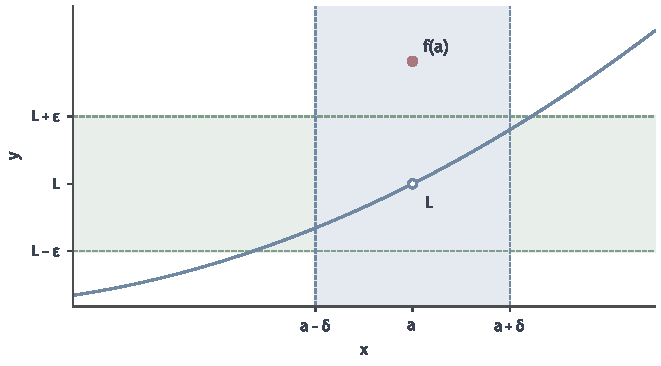
\includegraphics[width=112.0mm]{figures/01-mathematical-preliminaries-upper/00-shared/matplotlib/chapter3-concept-processes/epsilon-delta-band.pdf}
 \caption{取$a=L=1$（$L$即正文中的极限值$b$），$x\neq1$时$f(x)=x^2$，另令$f(1)=2$。蓝带对应$\delta=0.2$的输入范围，绿带对应$\varepsilon=0.55$的输出范围；去掉$a$后，蓝带内曲线全部落在绿带内。空心点是极限位置，红实心点是$f(a)$，不参加去心邻域条件。}
 \label{fig:analysis-process-epsilon-delta-band}
\end{figure}

\paragraph{单侧极限与无穷处的极限}
实轴上的输入可以从两侧接近一点，两侧的输出未必有相同趋向。只让$x<a$的输入趋近$a$，得到左极限$\lim_{x\to a^-}f(x)$；只让$x>a$的输入趋近，得到右极限$\lim_{x\to a^+}f(x)$。
两者分别在上述条件中加上$x<a$或$x>a$，并要求那一侧有定义域中的点任意靠近$a$。两侧都能趋近时，极限存在当且仅当左右极限都存在且相等。

例如阶跃函数$\mathbb I\{x\geq0\}$在$0$处的左极限为$0$、右极限为$1$，所以极限不存在。在闭区间$[a,b]$上，左端点只能从右侧趋近，右端点只能从左侧趋近，端点处的极限总是指单侧极限。

输入还可以趋向无穷。设定义域向右无界，$\lim_{x\to+\infty}f(x)=b$表示：对每个$\varepsilon>0$，存在$M$使定义域中所有$x>M$都满足$|f(x)-b|<\varepsilon$；$x\to-\infty$类似。

输出也可以越过任何有限界：对有限聚点$a$，$f(x)\to+\infty$（$x\to a$）表示对每个实数$M$都存在$\delta>0$，使定义域中满足$0<|x-a|<\delta$的$x$都有$f(x)>M$。
以$1/x$为例：$x\to\pm\infty$时它趋于$0$，这是输入趋向无穷；$x\to0^+$时它趋于$+\infty$，$x\to0^-$时趋于$-\infty$，这是输出趋向无穷，两侧方向不同，因而没有共同的双侧极限。

\paragraph{无穷小、无穷大与渐近记号}
\label{sec:comb-growth-scales}
趋向零的量出现在误差、余项和微分中，需要一个统一的名称。在指定的趋向下极限为$0$的函数或数列称为\term{无穷小}（infinitesimal），绝对值趋于$+\infty$的称为无穷大。

例如$x\to0$时$x$与$x^2$都是无穷小，$n\to\infty$时$1/n$是无穷小。无穷小描述的是一个变化过程的极限性质，不是某个固定的很小的数。若$f$在趋向附近非零，则$f$为无穷大当且仅当$1/f$为无穷小。

两个无穷小趋于零的相对速度可以不同，比较它们的比值即可。设在所讨论的趋向附近$g\neq0$。
\begin{definition}[渐近记号]
\label{def:ru-asymptotic-notation}
若$f/g\to0$，记$f=o(g)$，表示$f$相对于$g$可以忽略；若$|f/g|$在趋向附近有界，即存在常数$C$使最终$|f|\leq C|g|$，记$f=O(g)$；若$f/g\to1$，记$f\sim g$，称二者等价。
\end{definition}
例如$x\to0$时$x^2=o(x)$，$3x=O(x)$但不是$o(x)$，$x+x^2\sim x$。比值把这些记号与相对误差联系起来：$f\sim g$恰好说明用$g$近似$f$的相对误差$|f-g|/|g|$趋于零。

等价无穷小可以在乘除中互相替换：若$f\sim f_1$、$g\sim g_1$，则$fg/(f_1g_1)=(f/f_1)(g/g_1)\to1$。相减时却不行，因为主要部分可能相互抵消。
例如$x\to0$时$f(x)=x+x^2$与$g(x)=x$都等价于$x$，若把两者都换成$x$再相减会得到$0$，而实际上$f-g=x^2$。抵消以后，留下的是原先被忽略的高阶部分，必须保留更精细的展开才能判断。

同样的记号可用于$n\to\infty$的数列，用来比较增长的快慢。$3n+7=O(n)$、$n/10=O(n)$，但两个比值分别趋于$3$和$0.1$，都不是$o(n)$；$10\sqrt n=o(n)$，因为$10\sqrt n/n\to0$。

对最终为正的数列，若存在$c>0$使$a_n\geq cb_n$最终成立，记$a_n=\Omega(b_n)$；同时满足$O$与$\Omega$时记$a_n=\Theta(b_n)$，表示同一数量级。
$n=O(n^2)$也成立，所以大$O$只给出上界，不一定是精确的增长阶。后文描述算法的计算量时沿用这里的含义，比较的始终是两个数量的比值。
图~\ref{fig:vol1-add-asymptotic-ratios}画出了上面三个比值。

\begin{figure}[!htb]
 \centering
 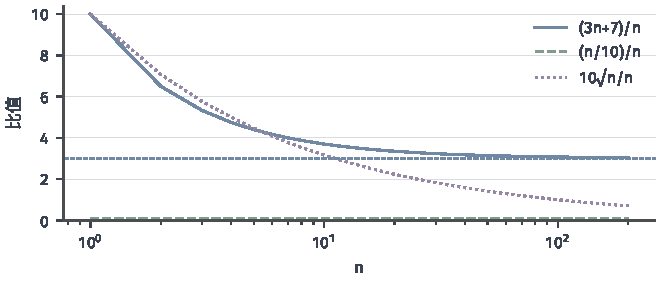
\includegraphics[width=112mm]{figures/01-mathematical-preliminaries-upper/00-shared/matplotlib/mathematical-language-combinatorics-analysis-optimization-comprehension-additions/asymptotic-ratios.pdf}
 \caption{三个解析数列除以$n$后的比值，展示整数$n=1,\ldots,200$，横轴为对数刻度。蓝、绿、紫线的极限分别为$3,0.1,0$。前两者对应$O(n)$而非$o(n)$，第三者对应$o(n)$；极限由正文中的表达式判断，有限范围曲线只帮助观察。}
 \label{fig:vol1-add-asymptotic-ratios}
\end{figure}

\subsection{函数极限存在的判别}
\label{sec:ru-function-limit-criteria}

函数极限要求控制$a$附近所有允许的输入，直接验证并不方便。下面的序列判据把它转化为数列极限，使上一节的工具可以直接使用。
\begin{theorem}[函数极限的序列判据]
\label{thm:ru-sequential-criterion}
设$a$为$X$的聚点。$\lim_{x\to a}f(x)=b$，当且仅当对每个满足$x_n\in X\setminus\{a\}$且$x_n\to a$的数列，都有$f(x_n)\to b$。
\end{theorem}
\begin{proof}
设函数极限为$b$。给定$\varepsilon$取相应的$\delta$，充分靠后的$x_n$满足$0<|x_n-a|<\delta$，于是$|f(x_n)-b|<\varepsilon$。

反过来用反证法。若误差条件不成立，就存在$\varepsilon_0>0$，使每个$\delta=1/n$都不合要求，即可选$x_n\in X$满足$0<|x_n-a|<1/n$而$|f(x_n)-b|\geq\varepsilon_0$；这列输入趋于$a$，输出却不趋于$b$。
\end{proof}
序列判据也是否定极限存在的常用工具：只要找到两列趋于$a$的输入，使输出趋于不同的值。例如$f(x)=\sin(1/x)$，沿$x_n=1/(2n\pi+\pi/2)$恒有$f(x_n)=1$，沿$y_n=1/(2n\pi+3\pi/2)$恒有$f(y_n)=-1$，所以$x\to0$时极限不存在。

不知道候选极限时，也可以像数列那样检查输出是否彼此接近。
\begin{theorem}[函数极限的柯西准则]
\label{thm:ru-function-cauchy}
设$a$为$X$的聚点。$x\to a$时$f(x)$有有限极限，当且仅当对每个$\varepsilon>0$，都存在$\delta>0$，使任意两个满足$0<|x-a|<\delta$、$0<|y-a|<\delta$的$x,y\in X$都有$|f(x)-f(y)|<\varepsilon$。
\end{theorem}
\begin{proof}
必要性由三角不等式得到：两个输出都与极限相差不到$\varepsilon/2$。

充分性先固定一列$x_n\in X\setminus\{a\}$、$x_n\to a$。对给定的$\varepsilon$，充分靠后的$x_n,x_m$都落在$\delta$去心邻域内，所以$(f(x_n))$是柯西数列，由实数的完备性收敛到某个$b$。
另取一列$y_n\to a$，把两列交错排成$x_1,y_1,x_2,y_2,\ldots$，它仍趋于$a$，输出列同样收敛；它的两个子列$(f(x_n))$与$(f(y_n))$必有同一极限。
所以每列趋于$a$的输入都给出同一个$b$，由序列判据，$f(x)\to b$。
\end{proof}
准则中的两个输入都不等于$a$，这与极限只看去心邻域的约定一致。数列的柯西准则依赖确界原理，这里通过它同样依赖实数的完备性。

\paragraph{极限的运算法则}
借助序列判据，数列极限的运算法则可以逐条搬到函数上。
\begin{theorem}[函数极限的运算法则]
\label{thm:ru-function-limit-laws}
设$a$为$X$的聚点，$f,g:X\to\mathbb R$，$x\to a$时$f(x)\to b$、$g(x)\to c$，其中$b,c\in\mathbb R$，$\lambda$为实常数，则$x\to a$时
\begin{enumerate}
 \item 和与差：$f(x)\pm g(x)\to b\pm c$；
 \item 数乘：$\lambda f(x)\to\lambda b$；
 \item 积：$f(x)g(x)\to bc$；
 \item 商：若$c\neq0$，则在$a$的某个去心邻域内$g\neq0$，并且$f(x)/g(x)\to b/c$。
\end{enumerate}
\end{theorem}
\begin{proof}
任取$x_n\in X\setminus\{a\}$、$x_n\to a$，由序列判据，$f(x_n)\to b$、$g(x_n)\to c$。对这两列数分别使用定理~\ref{thm:ru-sequence-limit-laws}中的和、差、数乘与积的法则，再由序列判据返回函数极限，即得前三条。

对商，先在$g$的极限定义中取$\varepsilon=|c|/2$，得到一个去心邻域，其中$|g(x)|>|c|/2>0$；在这个邻域内任取趋于$a$的输入列，用数列的商法则，再由序列判据返回。
\end{proof}
分子分母都趋于零时不能套用商的法则。例如$(x^2-1)/(x-1)$在$x\to1$时须先约去公因子$x-1$，才能求出极限$2$。

\begin{theorem}[函数极限的夹逼定理]
\label{thm:ru-function-squeeze}
若在$a$的某个去心邻域内，所有允许的输入都满足$u(x)\leq h(x)\leq v(x)$，且$x\to a$时$u(x)\to L$、$v(x)\to L$，其中$L\in\mathbb R$，则$h(x)\to L$。
\end{theorem}
\begin{proof}
任给$\varepsilon>0$，取一个共同的去心邻域，使其中$u(x)$与$v(x)$都落在$(L-\varepsilon,L+\varepsilon)$内，夹在中间的$h(x)$也在其中。
\end{proof}
例如$-|x|\leq x\sin(1/x)\leq|x|$，所以$x\to0$时$x\sin(1/x)\to0$。

复合函数的极限需要多一点小心。设$x\to a$时$f(x)\to b$，$y\to b$时$g(y)\to c$。若在$a$的某个去心邻域内$f(x)\neq b$，或者$g$在$b$处有定义且$g(b)=c$，则$g(f(x))\to c$。

没有这两个条件之一，结论可能失败：令$f\equiv b$为常数，$g(y)=1$（$y\neq b$）、$g(b)=0$，则$y\to b$时$g(y)\to1$，但$g(f(x))\equiv0$。
问题在于外层的极限只看$b$的去心邻域，而内层的输出可能恰好落在被排除的$b$上；第一个条件保证这种情形不发生，第二个条件则说明即使发生也没有影响。

\subsection{基本函数的极限}
\label{sec:ru-elementary-limits}

上一章把指数和三角函数当作已知对象。现在有了级数和函数极限，可以给出指数函数的定义，并求出后面计算导数要用的两个基本极限。

\paragraph{自然指数函数}
对每个实数$x$，级数$\sum_{k\geq0}x^k/k!$相邻项绝对值之比为$|x|/(k+1)\to0$，由比值判别绝对收敛。定义
\[
 \exp x=\sum_{k=0}^\infty\frac{x^k}{k!}.
\]

指数函数最重要的性质是加法公式$\exp(x+y)=\exp x\,\exp y$。证明要计算两个级数的乘积，先说明绝对收敛级数可以按总次数归并。

设$\sum_ka_k$与$\sum_jb_j$绝对收敛。有限的正方形和满足$\sum_{k,j\leq N}a_kb_j=(\sum_{k\leq N}a_k)(\sum_{j\leq N}b_j)$，因此趋于两个和的乘积。
按总次数$k+j=n\leq N$归并的三角形和，与正方形和只差满足$k,j\leq N$、$k+j>N$的项；这些项中$k$或$j$大于$N/2$，其绝对值之和不超过
$(\sum_{k>N/2}|a_k|)(\sum_j|b_j|)+(\sum_k|a_k|)(\sum_{j>N/2}|b_j|)$，它随$N$增大趋于零。所以按总次数归并后得到同一极限。

用于指数级数，第$n$组为$\sum_{k=0}^nx^ky^{n-k}/[k!(n-k)!]$，由二项式定理它等于$(x+y)^n/n!$，于是
\[
 \exp x\,\exp y=\sum_{n=0}^\infty\frac{(x+y)^n}{n!}=\exp(x+y).
\]
记$e=\exp1\approx2.71828$。由加法公式，对正整数$n$有$\exp n=e^n$，因此通常把$\exp x$写作$e^x$。

加法公式推出了上一章当作已知的几条性质。由$e^xe^{-x}=e^0=1$知$e^x\neq0$，又$e^x=(e^{x/2})^2\geq0$，所以$e^x>0$。
对$u\geq0$，级数各项非负，只保留前两项便得$e^u\geq1+u$；于是$h>0$时$e^{x+h}=e^xe^h\geq e^x(1+h)>e^x$，指数函数严格递增。
同一不等式说明$x\to+\infty$时$e^x\to+\infty$，再由$e^x=1/e^{-x}$得$x\to-\infty$时$e^x\to0$。

原点附近的变化可以直接从级数估计。当$0<|h|<1/2$时，由$1/k!\leq1$，
\[
 |e^h-1-h|\leq\sum_{k=2}^\infty|h|^k=\frac{h^2}{1-|h|}\leq2h^2.
\]
除以$|h|$得$|(e^h-1)/h-1|\leq2|h|$，因此
\[
 \lim_{h\to0}\frac{e^h-1}{h}=1.
\]
这一推导只用到级数的估计，没有用到导数或逐项求导。同一估计还给出$|e^{x+h}-e^x|=e^x|e^h-1|\leq e^x(|h|+2h^2)\to0$，下一节将据此说明指数函数连续，并构造它的反函数自然对数。

\paragraph{三角函数的基本极限}
三角函数的基本极限来自单位圆上的几何比较。设$0<h<\pi/2$，比较单位圆中以$h$为圆心角的内接三角形、扇形与外切三角形的面积，得到$\sin h\leq h\leq\tan h$，即
\[
 \cos h\leq\frac{\sin h}h\leq1.
\]
又由$1-\cos h=2\sin^2(h/2)\leq h^2/2$，得到$0\leq1-\sin h/h\leq h^2/2$。$\sin h/h$是偶函数，同一估计对$h<0$也成立，由夹逼定理，
\[
 \lim_{h\to0}\frac{\sin h}h=1,\qquad\lim_{h\to0}\frac{\cos h-1}h=0,
\]
后者来自$|1-\cos h|/|h|\leq|h|/2$。第一个极限恰为$1$，依赖于用弧长度量角；若用角度制，会多出比例系数$\pi/180$。

\section{连续性}
\label{sec:ru-continuity}
\label{sec:analysis-local-models}
\label{sec:analysis-metric-continuity-extrema}

对$f(x)=x^2$，输入$x$接近$a$时，输出接近$a^2$，而$a^2$恰好是函数在$a$处的值。连续性描述的就是这种关系：输出趋近的目标等于函数在该点的取值。
本节先给出定义和运算性质，再研究闭区间上的连续函数为什么一定达到最值、取遍中间值，最后比较几种强弱不同的连续性条件。

\subsection{连续性的定义和性质}
\label{sec:ru-continuity-definition}

\begin{definition}[连续]
\label{def:analysis-continuity}
设$X\subseteq\mathbb R$，$f:X\to\mathbb R$，$a\in X$。若对每个$\varepsilon>0$，都存在$\delta>0$，使
\[
 x\in X,\quad|x-a|<\delta\quad\Longrightarrow\quad|f(x)-f(a)|<\varepsilon,
\]
则称$f$在$a$处\term{连续}（continuous）。若$f$在$X$的每一点连续，就称$f$为连续函数。
\end{definition}
与函数极限的定义相比，这里不排除$x=a$，因为目标值就是$f(a)$。连续性与极限的关系取决于$a$在定义域中的位置。
若$a$是$X$的聚点，连续等价于$\lim_{x\to a}f(x)=f(a)$；若$a$是孤立点，取$\delta$足够小，使邻域内属于$X$的点只有$a$，条件自动成立；
若$a$是闭区间的端点，连续就是相应的单侧极限等于函数值。

用定义验证连续性时，需要对每个$\varepsilon$具体找出$\delta$。
\begin{example}[平方函数在每一点连续]
\label{ex:analysis-square-pointwise-continuity}
设$f(x)=x^2$，固定$a$。若$|x-a|<1$，则$|x+a|\leq|x-a|+2|a|<2|a|+1$，从而$|x^2-a^2|=|x-a|\,|x+a|\leq(2|a|+1)|x-a|$。
给定$\varepsilon>0$，取$\delta=\min\{1,\varepsilon/(2|a|+1)\}$，则$|x-a|<\delta$时$|x^2-a^2|<\varepsilon$。
\end{example}
例中的$\delta$随$|a|$增大而缩小：基点离原点越远，图像越陡，允许的输入误差越小。第~\ref{sec:analysis-continuity-relations}节将说明，在整条实轴上这种依赖无法消除。

不连续的点称为间断点，按失效方式可以分为几类。若$\lim_{x\to a}f(x)$存在但不等于$f(a)$，称为可去间断：改变$f(a)$的值，函数便连续，例如把$x^2$在$0$处的值改为$1$。
若左右极限都存在但不相等，称为跳跃间断，例如阶跃函数$\mathbb I\{x\geq0\}$在$0$处。两类并未穷尽所有情形：令$f(0)=0$、$x\neq0$时$f(x)=\sin(1/x)$，上一节已看到它在$0$处连单侧极限都不存在，这是振荡导致的间断。

连续性可以用序列刻画：$f$在$a\in X$处连续，当且仅当对每列满足$x_n\in X$、$x_n\to a$的输入，都有$f(x_n)\to f(a)$。证明与函数极限的序列判据相同，只是不必排除$x_n=a$。
由此，函数极限的运算法则直接给出：$f,g$在$a$处连续时，$f\pm g$、$fg$、$cf$在$a$处连续；若还有$g(a)\neq0$，则$f/g$在$a$附近有定义并在$a$处连续。
复合同样保持连续：若$f$在$a$处连续，$g$在$f(a)$处连续，则$g\circ f$在$a$处连续。给定$\varepsilon$，先由$g$的连续性得到$\eta$，再由$f$的连续性取$\delta$使$|f(x)-f(a)|<\eta$，两步误差传递便连成一步。
与复合函数的极限不同，这里外层在$f(a)$处连续，所以不需要额外条件。由这些规则，多项式在$\mathbb R$上连续，有理函数在分母非零处连续。
本节只用实轴上的绝对值距离；把输入和输出的距离换成一般的度量，就得到第~\ref{chap:metric-spaces}章中一般映射的连续性。

\subsection{闭区间上连续函数的性质}
\label{sec:ru-closed-interval-continuity}
\label{sec:analysis-metric-measurement}
\label{sec:analysis-set-metric}

函数$f(x)=x$在$(0,1)$上连续，却没有最小值；在$[0,1]$上则有。区别来自定义域：$(0,1)$中的点列$1/n$趋于$0$，极限却不在定义域内。
要从各点的局部性质得到整个定义域上的结论，需要先描述哪些集合能留住其中点列的极限，以及怎样把局部控制合成整体控制。

集合$U\subseteq\mathbb R$若对每个$x\in U$都存在$r>0$使$(x-r,x+r)\subseteq U$，就称为\term{开集}（open set）；补集为开集的集合称为\term{闭集}（closed set）。
开区间是开集，闭区间是闭集；$[0,1)$既不开也不闭，$\mathbb R$与空集既开又闭。闭集的意义可以换成点列的语言来理解。
\begin{lemma}[闭集的序列判据]
\label{lem:analysis-closed-sequence-criterion}
$F\subseteq\mathbb R$是闭集，当且仅当：每个取值于$F$的收敛数列，其极限也属于$F$。
\end{lemma}
\begin{proof}
设$F$闭。若取值于$F$的数列收敛到$x\notin F$，开集$\mathbb R\setminus F$包含某个$(x-r,x+r)$，充分靠后的项都落在其中，与$x_n\in F$矛盾。
反之，若$F$不闭，补集不是开集，存在$x\notin F$使每个$(x-1/n,x+1/n)$都与$F$相交；从中各选一点$x_n\in F$，则$x_n\to x\notin F$。
\end{proof}
闭与有界是不同的性质：$(0,1)$有界但不闭，$\mathbb R$闭但无界。二者同时成立时，Bolzano--Weierstrass定理给出收敛子列，本引理又保证子列的极限仍在集合内。
这一“闭有界集中的点列有收敛到集合内的子列”的性质，是本小节各定理的共同依据。

同一性质还有另一种表达：把局部控制合成整体控制。若一族开集的并包含$K$，称它们为$K$的\term{开覆盖}（open cover）；若能从中选出有限个仍覆盖$K$，称为\term{有限子覆盖}（finite subcover）。
若$K$的每个开覆盖都有有限子覆盖，称$K$\term{紧致}（compact）。
\begin{theorem}[闭区间的有限子覆盖性质]
\label{thm:analysis-interval-finite-subcover}
实轴上的每个闭区间$[a,b]$都是紧致集。
\end{theorem}
\begin{proof}
设$a<b$，给定$[a,b]$的开覆盖$\mathcal U$。先证明存在一个共同尺度：
\begin{equation}
 \exists r>0,\quad\forall x\in[a,b],\quad\exists U\in\mathcal U,\qquad(x-r,x+r)\cap[a,b]\subseteq U.
 \label{eq:analysis-cover-uniform-radius}
\end{equation}
若不然，对每个$n$可选$x_n\in[a,b]$，使$(x_n-1/n,x_n+1/n)\cap[a,b]$不包含于任何覆盖成员。取收敛子列$x_{n_k}\to x\in[a,b]$，选$U\in\mathcal U$与$\rho>0$使$(x-\rho,x+\rho)\subseteq U$。
当$k$足够大时$|x_{n_k}-x|<\rho/2$且$1/n_k<\rho/2$，于是$(x_{n_k}-1/n_k,x_{n_k}+1/n_k)\subseteq U$，与选取矛盾。
有了共同半径$r$，把$[a,b]$分成有限个长度小于$r$的小段，每段落在某个$(x-r,x+r)$内，因而被一个覆盖成员包含；每段选一个成员即得有限子覆盖。
\end{proof}
图~\ref{fig:analysis-process-finite-open-cover}对照闭区间的有限覆盖与开区间上无法有限选取的覆盖。每个有界闭集也是紧致的：把它放进某个$[a,b]$，把它的补集加入开覆盖，应用定理后再删去补集即可。
有限子覆盖与收敛子列是同一性质的两种说法，后者在下面的证明中更直接，前者在需要把无限多个局部估计合成一个时更方便。

\begin{figure}[!htbp]
 \centering
 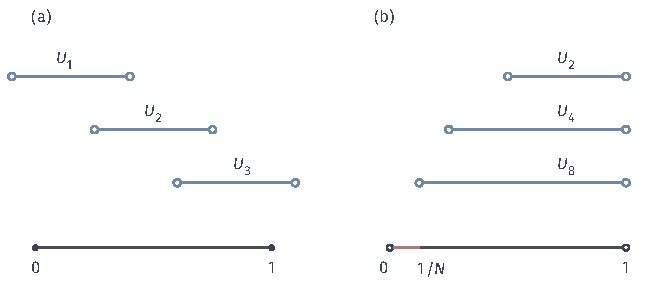
\includegraphics[width=112mm]{figures/01-mathematical-preliminaries-upper/00-shared/tikz/chapter3-concept-processes/finite-open-cover.pdf}
 \caption{(a) 三个开区间$(-0.1,0.4)$、$(0.25,0.75)$、$(0.6,1.1)$覆盖$[0,1]$。(b) $U_n=(1/n,1)$（$n\geq2$）覆盖$(0,1)$；只选有限多个时，设最大下标为$N$，红段$(0,1/N]$仍未覆盖。图只画$U_2,U_4,U_8$；右侧的失败由最大下标论证，不是有限图像的猜测。}
 \label{fig:analysis-process-finite-open-cover}
\end{figure}

\begin{theorem}[极值定理]
\label{thm:analysis-extreme-value}
设$K\subseteq\mathbb R$非空、闭且有界，$f:K\to\mathbb R$连续，则$f$有界，并在$K$上达到最小值和最大值。
\end{theorem}
\begin{proof}
若$f$无界，可选$x_n\in K$使$|f(x_n)|>n$；取收敛子列$x_{n_k}\to x\in K$，连续性给出$f(x_{n_k})\to f(x)$，收敛数列有界，与$|f(x_{n_k})|>n_k$矛盾。
于是$m=\inf_Kf$是有限实数。对每个$n$选$x_n\in K$使$m\leq f(x_n)<m+1/n$，取收敛子列$x_{n_k}\to x^\star\in K$，则$f(x_{n_k})\to f(x^\star)$，同时$f(x_{n_k})\to m$，所以$f(x^\star)=m$。对$-f$重复论证即得最大值。
\end{proof}
三个条件各排除一种失效方式：有界保证收敛子列，闭保证子列的极限仍在定义域内，连续保证函数值随之收敛。下面三个例子各缺一个条件，下确界都取不到。
\begin{example}[极值定理的条件]
\label{ex:analysis-extrema-failures}
定义域不闭：$f(x)=x$在$(0,1)$上的下确界$0$不被取得。定义域无界：$e^x$在$\mathbb R$上连续，下确界为$0$，但$e^x>0$，取不到。
函数不连续：在$[0,1]$上令$f(0)=1$、$x>0$时$f(x)=x$，下确界为$0$，而$f$在每一点的值都大于$0$。
\end{example}

另一条整体性质说的是：函数从一个值变到另一个值时，要经过中间的每个值。这要求两端之间的整段都属于定义域。
\begin{theorem}[介值定理]
\label{thm:analysis-intermediate-value}
设$a<b$，$f:[a,b]\to\mathbb R$连续。则对介于$f(a)$与$f(b)$之间的每个$c$，都存在$\xi\in[a,b]$使$f(\xi)=c$；若$c$严格位于二者之间，可取$\xi\in(a,b)$。
\end{theorem}
\begin{proof}
设$f(a)<c<f(b)$（端点值相等的情形直接取端点，$f(a)>f(b)$时考虑$-f$）。令$S=\{x\in[a,b]:f(x)\leq c\}$，它含$a$且以$b$为上界，由确界原理$u=\sup S$存在。
取$x_n\in S$使$x_n\to u$，连续性给出$f(u)\leq c$，因而$u\neq b$。若$f(u)<c$，由连续性，$u$右侧充分近的点仍满足$f<c$，它们属于$S$却大于$u$，矛盾。所以$f(u)=c$，又由$f(a)<c$知$u\neq a$。
\end{proof}
证明用到了区间不缺中间点：确界$u$仍在区间中，并且$u$的右侧还有区间内的点。定义域闭且有界但有缺口时，介值性可能失效。
\begin{example}[有缺口的定义域上不取中间值]
\label{ex:analysis-intermediate-value-gap}
令$X=[-2,-1]\cup[1,2]$，在$[-2,-1]$上取$f=0$，在$[1,2]$上取$f=1$。对每个$a\in X$取$\delta=1$，邻域内属于$X$的点与$a$在同一段，所以$f$连续。$X$闭且有界，$f$却不取$1/2$。
\end{example}
这个函数在$X$上仍然达到最值：闭有界足以保证最值，却不能代替介值定理的区间条件。

介值定理最直接的用途是证明方程有解。若$f$在$[a,b]$上连续且$f(a)f(b)<0$，则$f$在$(a,b)$内有零点。这个结论还给出求零点的方法，即\term{二分法}（bisection method）：
取中点$m=(a+b)/2$，若$f(m)=0$则停止，否则保留端点函数值异号的那一半，重复进行。$n$步后零点落在长度为$(b-a)/2^n$的区间内，取该区间中点作为近似值，误差不超过$(b-a)/2^{n+1}$。
例如$f(x)=x^2-2$在$[1,2]$上两端异号，第一步$f(1.5)=0.25>0$保留$[1,1.5]$，第二步$f(1.25)<0$保留$[1.25,1.5]$；要使误差小于$10^{-6}$，约需$20$步。
二分法只用到连续性和符号，不需要导数；所需步数由误差界事先确定。

介值定理还说明，区间上的连续函数把区间映成区间：若$f(I)$中有$y_1<y_2$，它们之间的每个值也被取到。由此可以研究反函数的连续性。
\begin{theorem}[严格单调连续函数的反函数]
\label{thm:ru-inverse-continuity}
\label{sec:analysis-inverse-continuity}
设$f$在区间$I$上连续且严格单调，则$f(I)$是区间，$f:I\to f(I)$是双射，并且反函数$f^{-1}$在$f(I)$上连续、与$f$同向严格单调。
\end{theorem}
\begin{proof}
双射与单调性已在第~\ref{sec:ru-function-properties}节说明，$f(I)$是区间由介值定理得到。以严格递增、$a$为$I$的内点为例，给定足够小的$\varepsilon>0$使$a\pm\varepsilon\in I$，有$f(a-\varepsilon)<f(a)<f(a+\varepsilon)$。
取$\delta=\min\{f(a)-f(a-\varepsilon),\,f(a+\varepsilon)-f(a)\}$，若$y\in f(I)$且$|y-f(a)|<\delta$，则$f(a-\varepsilon)<y<f(a+\varepsilon)$，严格递增迫使$f^{-1}(y)\in(a-\varepsilon,a+\varepsilon)$。端点只在一侧取点，论证相同。
\end{proof}

现在可以严格构造自然对数。上一节已经得到：$e^x$严格递增，$x\to-\infty$时趋于$0$，$x\to+\infty$时趋于$+\infty$，并且$|e^{x+h}-e^x|\leq e^x(|h|+2h^2)$，所以它在每一点连续。
对任意$y>0$，先取两个输入使指数值分别小于和大于$y$，再用介值定理得到原像；严格单调保证原像唯一。所以$e^x$是$\mathbb R$到$(0,+\infty)$的双射，它的反函数称为\term{自然对数}（natural logarithm），记作$\log x$，定义在$x>0$上。
由定理~\ref{thm:ru-inverse-continuity}，$\log$连续且严格递增；由指数的加法公式，$\log(xy)=\log x+\log y$。对$a>0$与实数$x$，定义$a^x=e^{x\log a}$，它对整数$x$与通常的乘幂一致。
这样，上一章作为背景使用的指数—对数关系，现在都有了依据。

\subsection{一致连续与Lipschitz连续}
\label{sec:ru-uniform-lipschitz}
\label{sec:analysis-continuity-relations}

连续性定义中的$\delta$可以随基点改变，平方函数的例子中$\delta$就随$|a|$增大而缩小。若要求同一个$\delta$适用于整个定义域，或者要求输出误差不超过输入误差的固定倍数，就得到更强的条件。
\begin{definition}[一致连续]
\label{def:analysis-uniform-continuity}
函数$f:X\to\mathbb R$称为\term{一致连续}（uniformly continuous），若对每个$\varepsilon>0$，都存在$\delta>0$，使任意$x,y\in X$满足$|x-y|<\delta$时都有$|f(x)-f(y)|<\varepsilon$。
\end{definition}
与逐点连续相比，变化在于量词的次序：逐点连续是“对每个点和每个$\varepsilon$，存在$\delta$”，一致连续是“对每个$\varepsilon$，存在对所有点都有效的$\delta$”。
\begin{example}[平方函数在实轴上不一致连续]
\label{ex:analysis-square-not-uniformly-continuous}
取$x_n=n$、$y_n=n+1/n$，则$|y_n-x_n|=1/n\to0$，而$y_n^2-x_n^2=2+1/n^2>2$。若平方函数在$\mathbb R$上一致连续，对$\varepsilon=1$取$\delta$，当$n>1/\delta$时便与上式矛盾。
\end{example}
两列点都逃向无穷远，那里平方函数越来越陡。把定义域限制在$[0,1]$上，则$|x^2-y^2|=|x+y|\,|x-y|\leq2|x-y|$，取$\delta=\varepsilon/2$即可。
同一个函数在两个定义域上表现不同，原因在于逃向无穷远的点列在有界闭集中不存在。
\begin{theorem}[一致连续性定理]
\label{thm:analysis-uniform-continuity}
设$K\subseteq\mathbb R$非空、闭且有界，$f:K\to\mathbb R$连续，则$f$在$K$上一致连续。特别地，闭区间上的连续函数一致连续。
\end{theorem}
\begin{proof}
若不然，存在$\varepsilon_0>0$，使每个$\delta=1/n$都对应$x_n,y_n\in K$，满足$|x_n-y_n|<1/n$而$|f(x_n)-f(y_n)|\geq\varepsilon_0$。
取收敛子列$x_{n_k}\to x\in K$，则$y_{n_k}\to x$。由$f$在$x$处连续，$f(x_{n_k})$与$f(y_{n_k})$都趋于$f(x)$，两者之差趋于零，与$\varepsilon_0$矛盾。
\end{proof}

一致连续只断言共同的$\delta$存在，没有给出输出误差与输入误差的数量关系。若这个关系是线性的，误差控制就更具体。
\begin{definition}[Lipschitz连续]
\label{def:analysis-lipschitz-continuity}
若存在常数$L\geq0$，使所有$x,y\in X$都满足
\begin{equation}
 |f(x)-f(y)|\leq L|x-y|,
 \label{eq:analysis-lipschitz-condition}
\end{equation}
则称$f$为\term{Lipschitz连续}（Lipschitz continuous）函数，$L$称为一个Lipschitz常数。若每一点都有一个邻域，$f$在其中满足这一条件（常数可随邻域改变），称$f$\term{局部Lipschitz连续}（locally Lipschitz）。
\end{definition}
Lipschitz连续蕴含一致连续：$L>0$时取$\delta=\varepsilon/L$即可。平方函数在$[0,1]$上可取$L=2$；在$\mathbb R$上割线斜率$x+y$无界，没有全局常数，
但在$(a-r,a+r)$内$|x+y|<2(|a|+r)$，所以它局部Lipschitz连续。

反过来，一致连续不蕴含Lipschitz连续。$\sqrt x$在$[0,1]$上连续，由一致连续性定理一致连续；但若有常数$L$，取$y=0$得$\sqrt x\leq Lx$，即$1/\sqrt x\leq L$对所有$x\in(0,1]$成立，这不可能。
它在零点附近的割线斜率无界。于是在同一个闭区间上有严格的强弱次序：Lipschitz连续强于一致连续，一致连续与连续等价；在无界区间上，连续又严格弱于一致连续。
比较时必须同时写明函数和定义域。控制许多短区间上总变化的绝对连续性，与积分能否恢复函数的问题相连，放在第~\ref{chap:measurable-functions}章讨论。

\section{函数列与函数项级数}
\label{sec:ru-function-sequences}

前几节的极限对象都是数。很多时候，我们用一系列函数逐步逼近同一个对象：几何级数的部分和$1+x+\cdots+x^N$逼近$1/(1-x)$，指数级数的部分和逼近$e^x$。
这时每个编号$n$对应一整个函数$f_n:X\to\mathbb R$，$(f_n)$称为\term{函数列}（sequence of functions）。
固定编号，看到的是一个函数；固定输入$x$，看到的是一列数$(f_n(x))_{n\geq1}$。函数列的收敛可以从后一个角度出发，但我们还关心收敛对整个函数意味着什么。

函数项级数$\sum_kg_k$的部分和$S_N=\sum_{k\leq N}g_k$本身就是一个函数列，级数的收敛与和函数都由部分和的极限决定。
所以下文先对函数列建立结论，再把它们用于部分和，不另建一套收敛语言。

\subsection{逐点收敛与一致收敛}
\label{sec:ru-pointwise-uniform}

最直接的做法是在每个输入处分别取数列极限。若对每个$x\in X$，数列$(f_n(x))$都收敛到$f(x)$，称$f_n$在$X$上\term{逐点收敛}（pointwise convergence）到$f$。
按数列极限的定义，这是说：对每个$x$和每个$\varepsilon>0$，存在$N$使$n\geq N$时$|f_n(x)-f(x)|<\varepsilon$，其中$N$可以随$x$改变。
若要求一个尾部起点同时控制全部输入，就得到更强的条件。
\begin{definition}[一致收敛]
\label{def:ru-uniform-convergence}
若对每个$\varepsilon>0$，都存在$N$，使$n\geq N$时对\emph{所有}$x\in X$都有$|f_n(x)-f(x)|<\varepsilon$，称$f_n$在$X$上\term{一致收敛}（uniform convergence）到$f$。
\end{definition}
两种收敛的差别与连续和一致连续的差别相同，都在于量词次序：$N$是否允许随$x$改变。

$f_n(x)=x^n$在$[0,1]$上的行为说明了这种差别。$0\leq x<1$时$x^n\to0$，$x=1$时恒为$1$，所以$f_n$逐点收敛到函数$f$，$f$在$[0,1)$上为$0$、在$1$处为$1$。
但在$x$接近$1$的地方，要使$x^n<1/2$，需要$n>\log2/\log(1/x)$，这个下界在$x\to1^-$时无界，没有一个$N$能同时管住所有$x$。
图~\ref{fig:ru-power-sequence-nonuniform}画出了几条$x^n$：无论$n$多大，曲线在靠近$1$处都要从接近$0$升到$1$，最大误差始终不小。

\begin{figure}[!htbp]
 \centering
 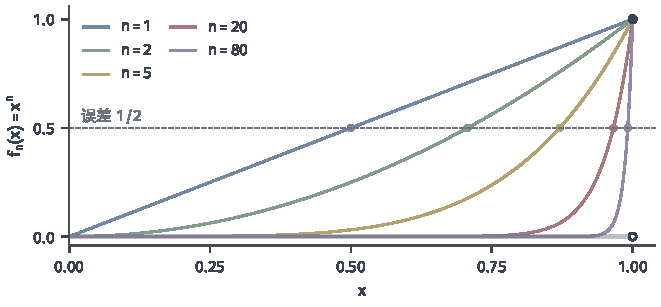
\includegraphics[width=112mm]{figures/01-mathematical-preliminaries-upper/02-real-numbers-and-univariate-functions/matplotlib/power-sequence-nonuniform/figure.pdf}
 \caption{函数列$f_n(x)=x^n$在$[0,1]$上的几条曲线（$n=1,2,5,20,80$）。逐点极限在$[0,1)$上为$0$（灰色水平线），在$x=1$处为$1$（实心点）。虚线标出误差$1/2$：每条曲线都在$x=2^{-1/n}$处越过它，越过位置随$n$增大逼近$1$，所以$\sup_{[0,1)}|f_n-f|=1$，收敛不一致。图为解析示例。}
 \label{fig:ru-power-sequence-nonuniform}
\end{figure}

\paragraph{一致收敛的判别}
直接检查一致收敛的办法是看最大误差。记$\|f_n-f\|_\infty=\sup_{x\in X}|f_n(x)-f(x)|$，则$f_n$一致收敛到$f$，当且仅当这个数列趋于零：两者说的都是“误差界可以对全部输入同时缩小”。
对$x^n$，在$[0,1)$上$\sup|x^n-0|=1$，不趋于零，所以收敛不一致；但在$[0,\rho]$（$\rho<1$）上，最大误差为$\rho^n\to0$，收敛是一致的。
可见一致收敛也依赖定义域，问题只出在$x=1$附近。这里的$\sup$只是一列数值的上确界，我们并没有把函数当作某个空间中的点。

不知道极限函数时，也可以用柯西条件检验。
\begin{theorem}[一致柯西准则]
\label{thm:ru-uniform-cauchy}
函数列$(f_n)$在$X$上一致收敛到某个函数，当且仅当对每个$\varepsilon>0$，存在$N$，使$m,n\geq N$时对所有$x\in X$都有$|f_m(x)-f_n(x)|<\varepsilon$。
\end{theorem}
\begin{proof}
必要性由三角不等式得到。对充分性，每个固定的$x$处$(f_n(x))$是柯西数列，因此收敛，记极限为$f(x)$。
在$|f_m(x)-f_n(x)|<\varepsilon$中固定$n\geq N$与$x$，令$m\to\infty$，得到$|f(x)-f_n(x)|\leq\varepsilon$，这个界对所有$x$同时成立。
\end{proof}

把一致柯西准则用于部分和，得到函数项级数最常用的判别法：用一列可求和的数值上界控制各项。
\begin{theorem}[Weierstrass判别法]
\label{thm:ru-weierstrass-m-test}
若存在非负数$M_k$，使$|g_k(x)|\leq M_k$对所有$x\in X$和$k$成立，且$\sum M_k<\infty$，则$\sum_kg_k$在$X$上一致收敛，并且对每个$x$绝对收敛。
\end{theorem}
\begin{proof}
对$m>n$，$|S_m(x)-S_n(x)|\leq\sum_{k=n+1}^m|g_k(x)|\leq\sum_{k>n}M_k$，右侧与$x$无关且随$n$增大趋于零，由一致柯西准则即得一致收敛；每个$x$处的绝对收敛由比较判别得到。
\end{proof}
例如$\sum_k\sin(kx)/k^2$在$\mathbb R$上一致收敛，可取$M_k=1/k^2$。第~\ref{sec:ru-power-series}节将用这一判别法证明幂级数在内部闭子区间上一致收敛。

\subsection{函数列连续性的保持}
\label{sec:ru-uniform-limit-continuity}

$x^n$的例子中，每个$f_n$都连续，逐点极限却在$1$处跳跃。所以逐点收敛不能保持连续性。一致收敛补上了缺失的一步。
\begin{theorem}[一致极限保持连续]
\label{thm:ru-uniform-limit-continuity}
若每个$f_n$在$a\in X$处连续，且$f_n$在$X$上一致收敛到$f$，则$f$在$a$处连续。特别地，连续函数列的一致极限是连续函数。
\end{theorem}
\begin{proof}
给定$\varepsilon>0$，由一致收敛选$n$使$|f_n(x)-f(x)|<\varepsilon/3$对所有$x$成立；再由$f_n$在$a$处连续选$\delta$，使$|x-a|<\delta$时$|f_n(x)-f_n(a)|<\varepsilon/3$。于是
\[
 |f(x)-f(a)|\leq|f(x)-f_n(x)|+|f_n(x)-f_n(a)|+|f_n(a)-f(a)|<\varepsilon.
\]
\end{proof}
证明把总误差拆成三段：两次用$f_n$逼近$f$的误差，以及固定函数$f_n$自身的连续误差。关键在于第一段和第三段用的是同一个$n$，并且这个$n$对点$x$和点$a$同时有效。
逐点收敛时，能让$|f_n(x)-f(x)|$变小的$n$可能随$x$改变，$x$越靠近$a$，所需的$n$越大，三段误差就无法同时控制；$x^n$在$1$附近正是这种情况。

把定理用于部分和：若每个$g_k$连续，且$\sum g_k$在$X$上一致收敛，则和函数连续，因为部分和是有限个连续函数之和。
结合Weierstrass判别法，$\sum\sin(kx)/k^2$的和函数在$\mathbb R$上连续。至于求导、积分能否与这种极限交换，分别留到第~\ref{sec:ru-termwise-differentiation}节与第~\ref{sec:ru-termwise-integration}节。

\section{幂级数}
\label{sec:ru-power-series}

在一般的函数项级数中，有一类各项由同一中心的整数次幂组成：
\[
 \sum_{k=0}^\infty c_k(x-x_0)^k,
\]
称为以$x_0$为中心的\term{幂级数}（power series），$c_k$称为系数。它的部分和是多项式，多项式只用加法和乘法就能计算，这使幂级数成为表示和近似函数的基本工具。
本节研究幂级数在哪些输入处收敛，以及收敛怎样控制和函数的连续性。

前面已经遇到两个幂级数：几何级数$\sum_kx^k$在$|x|<1$时收敛到$1/(1-x)$，指数级数$\sum_kx^k/k!$在每个实数处收敛。对收敛的输入，级数的和定义了一个函数，称为和函数。
几何级数在$|x|\geq1$时发散，可见幂级数未必处处收敛。下面先确定收敛的输入范围，再研究在什么范围内能对全部输入统一控制误差。已有函数怎样展开成幂级数，留到第~\ref{sec:ru-elementary-taylor}节。

\subsection{收敛半径与收敛区间}
\label{sec:ru-radius-of-convergence}

先看一点处的收敛对其他输入意味着什么。下面的结论说明，幂级数的收敛范围总是关于中心对称的一段（可能还包括端点）。
\begin{theorem}[Abel第一定理]
\label{thm:ru-abel-lemma}
若幂级数$\sum c_k(x-x_0)^k$在某点$x_1\neq x_0$处收敛，记$r=|x_1-x_0|$，则它在每个满足$|x-x_0|<r$的$x$处绝对收敛。
\end{theorem}
\begin{proof}
$x_1$处的级数收敛，所以其项趋于零，进而有界：存在$M$使$|c_k|r^k\leq M$对所有$k$成立。对$|x-x_0|<r$，记$q=|x-x_0|/r<1$，则
\[
 |c_k(x-x_0)^k|=|c_k|r^kq^k\leq Mq^k,
\]
与收敛的几何级数$\sum Mq^k$比较，即得绝对收敛。
\end{proof}
取逆否命题：若级数在某点$x_2$处发散，则它在每个离中心更远的点$x$（$|x-x_0|>|x_2-x_0|$）处也发散；否则那一点的收敛会推出$x_2$处收敛。

于是令$R=\sup\{|x-x_0|:\text{级数在}x\text{处收敛}\}\in[0,+\infty]$，称为\term{收敛半径}（radius of convergence）。由Abel第一定理，$|x-x_0|<R$时级数绝对收敛，$|x-x_0|>R$时级数发散。
$R=0$时级数只在中心处收敛；$R=+\infty$时在整条实轴上收敛；$0<R<+\infty$时，开区间$(x_0-R,x_0+R)$称为收敛区间，在其中绝对收敛，在其外发散。
两个端点$x_0\pm R$处的行为定理没有给出，必须各自检验。实际收敛的输入组成的集合称为收敛域，它是收敛区间加上收敛的端点。

\paragraph{收敛半径的计算}
收敛半径可以由系数算出。对固定的$x$，把根值判别用于$\sum|c_k|\,|x-x_0|^k$：$\limsup(|c_k|\,|x-x_0|^k)^{1/k}=|x-x_0|\limsup|c_k|^{1/k}$，它小于$1$时收敛，大于$1$时发散。由此得到
\[
 \frac1R=\limsup_{k\to\infty}|c_k|^{1/k},
\]
称为Cauchy--Hadamard公式，约定右侧为$0$时$R=+\infty$、为$+\infty$时$R=0$。
若系数非零且$|c_{k+1}/c_k|\to\ell$，用比值判别同样得到$R=1/\ell$，计算往往更方便。比值算法要求相邻系数非零且比值有极限；不满足时仍可用Cauchy--Hadamard公式。
例如$\sum x^{2k}$的奇数次系数为零，相邻系数之比没有定义，但$|c_k|^{1/k}$在偶数$k$处为$1$、奇数$k$处为$0$，上极限为$1$，所以$R=1$。

几个例子说明公式怎样用，也说明半径不能代替端点判别。指数级数的系数比为$1/(k+1)\to0$，$R=+\infty$；$\sum k!\,x^k$的系数比$k+1\to\infty$，$R=0$，只在$x=0$处收敛。
$\sum x^k$、$\sum x^k/k$、$\sum x^k/k^2$的收敛半径都是$1$，端点行为却各不相同：第一个在$x=\pm1$处都发散，收敛域为$(-1,1)$；
第二个在$x=1$处是调和级数，发散，在$x=-1$处是交错调和级数的相反数，条件收敛，收敛域为$[-1,1)$；第三个在两端都绝对收敛，收敛域为$[-1,1]$。

\subsection{区间内的一致收敛性}
\label{sec:ru-power-series-uniform}

在整个收敛区间上未必能统一控制误差。几何级数截断到第$N$项的误差为$|x|^{N+1}/|1-x|$，在$[-\rho,\rho]$（$\rho<1$）上不超过$\rho^{N+1}/(1-\rho)$，可以用一个$N$同时控制；
在整个$(-1,1)$上，$x\to1^-$时误差趋于无穷，不存在共同的$N$。退一步，在严格位于收敛区间内部的闭子区间上，统一控制总是可以做到的。

\paragraph{内闭一致收敛}
设$R>0$，取$0<\rho<R$。在$|x-x_0|\leq\rho$上，$|c_k(x-x_0)^k|\leq|c_k|\rho^k$；而$x_0+\rho$位于收敛区间内部，级数在那里绝对收敛，即$\sum|c_k|\rho^k<\infty$。
由Weierstrass判别法，幂级数在$[x_0-\rho,x_0+\rho]$上一致收敛。由于$\rho$可以任意接近$R$，收敛区间内的每个闭子区间都含于某个这样的区间，这称为内闭一致收敛。
它不等于在整个开区间上一致收敛：几何级数在$(-1,1)$上的最大误差为无穷。

\paragraph{端点处的一致收敛}
端点的情形需要另外处理。若$0<R<\infty$且级数在端点$x_0+R$处收敛，那么在从中心到这个端点的整个闭区间上都可以统一控制误差，即使端点处只是条件收敛。
\begin{theorem}[Abel第二定理]
\label{thm:ru-abel-endpoint}
设$0<R<\infty$。若$\sum c_kR^k$收敛，则幂级数$\sum c_k(x-x_0)^k$在$[x_0,x_0+R]$上一致收敛。另一端$x_0-R$有对称的结论；两端都收敛时，在整个$[x_0-R,x_0+R]$上一致收敛。
\end{theorem}
\begin{proof}
令$t=(x-x_0)/R\in[0,1]$，$a_k=c_kR^k$，只需证明$\sum a_kt^k$在$[0,1]$上一致收敛。记$A_{n,m}=\sum_{k=n}^ma_k$。由$\sum a_k$收敛与柯西准则，给定$\varepsilon>0$，存在$N$使$m\geq n\geq N$时$|A_{n,m}|<\varepsilon$。
用第~\ref{sec:ru-series-tests}节的有限分部求和，令$A_{n,n-1}=0$，
\[
 \sum_{k=n}^ma_kt^k=A_{n,m}t^m+\sum_{k=n}^{m-1}A_{n,k}(t^k-t^{k+1}).
\]
$t\in[0,1]$时$t^k-t^{k+1}\geq0$，这些差的和为$t^n-t^m$，所以右侧绝对值不超过$\varepsilon t^m+\varepsilon(t^n-t^m)=\varepsilon t^n\leq\varepsilon$。
这一估计对所有$t\in[0,1]$同时成立，由一致柯西准则即得一致收敛。
\end{proof}
定理只要求端点处的数值级数收敛，允许它条件收敛；结论也只涉及收敛的那一端，不能推到发散的另一端。

\paragraph{和函数的连续性}
把这两个结论与上一节的连续性定理结合，就得到和函数的连续性。幂级数的各项是多项式，都连续。收敛区间内的每一点都落在某个内部闭子区间中，部分和在那里一致收敛，所以和函数在该点连续。

若$0<R<\infty$且某个端点包含在收敛域中，Abel第二定理给出从中心到该端点的一致收敛，和函数在该端点单侧连续（端点只能从区间内部趋近）。$R=0$时收敛域只有中心一点，单点定义域上的函数自动连续。
所以幂级数的和函数在实际收敛域内处处连续。

两个例子标出了结论的范围。几何级数在两个端点都发散，端点不在收敛域中，结论自然不涉及它们；事实上$x\to1^-$时和函数$1/(1-x)\to+\infty$，无法延伸到端点。
$\sum x^k/k$在$x=-1$处收敛，由Abel第二定理，它的和函数在$[-1,1)$上连续，在$-1$处右连续。第~\ref{sec:ru-elementary-taylor}节将证明这个和函数是$-\log(1-x)$，由$-1$处的连续性便得到交错调和级数的和为$\log2$。


\FloatBarrier
\section{本章小结}
\label{sec:function-limits-summary}

本章处理了四类问题。求极限，靠的是极限的四则运算、夹逼和序列判据，它们都以有限极限已经存在为前提。
保证极限存在，靠的是单调有界、收敛子列和柯西准则，三者都回到实数的完备性；有理数中这些结论都会失效。
控制误差，靠的是余项估计：几何级数和交错级数的余项可以写出上界，Weierstrass判别法用可求和的数值上界控制整列函数。
交换操作，例如交换极限与连续性、交换求和次序，则需要额外的统一控制：绝对收敛允许任意重排，一致收敛保持连续性，逐点收敛和条件收敛都不够。

连续性把输入的趋近与输出的趋近联系起来。闭区间上的连续函数有界、达到最值、取遍中间值，并且一致连续；
这些整体性质分别依赖定义域有界、闭和不缺中间点。幂级数在收敛半径以内绝对收敛，在内部闭子区间上一致收敛，和函数在实际收敛域内连续。
连续还不保证可微，有限累计也尚未推广为一般的积分。下一章研究变化率，再下一章研究累计；两章都直接使用这里的连续性与闭区间性质，不再重新建立。
